\subsection{Progettazione di dettaglio e codifica}
Il periodo di progettazione di dettaglio e codifica comincia il 2019-03-16 e si conclude il 2019-04-19. L'inizio coincide con il giorno successivo alla consegna dei documenti per la Revisione di Progettazione. La conclusione coincide con la consegna dei documenti per la Revsione di Qualità. 
\subsubsection{Incrementi}
In questo periodo si effettuano 4 incrementi e le attività principali sono:
\begin{itemize}
\item{\textbf{Correzione e verifica}: vengono corretti e verificati i documenti necessari in base a quanto emerso dalla Revisione di Progettazione. Inoltre simigliora e si aggiorna il documento contenente il \emph{Glossario};} 
\item{\textbf{\gl{Product Baseline}}: questa attività definisce i dettaglio la struttura e le componenti del prodotto, attenendosi a quanto riportato in \emph{Tecnology Baseline};} 
\item{\textbf{Codifica}: i programmatori iniziano lo sviluppo del codice del prodotto, attenendosi a quanto riportato in \emph{Product Baseline};}	
\item{\textbf{Manuale utente}: attività che prevede la stesura di tutti i documenti volti a definire le linee guida per l'utilizzo del sistema.}
\end{itemize}

\subsubsection{Progettazione di dettaglio e codifica - Gantt delle attività}

\begin{figure} [H]
	\centering
	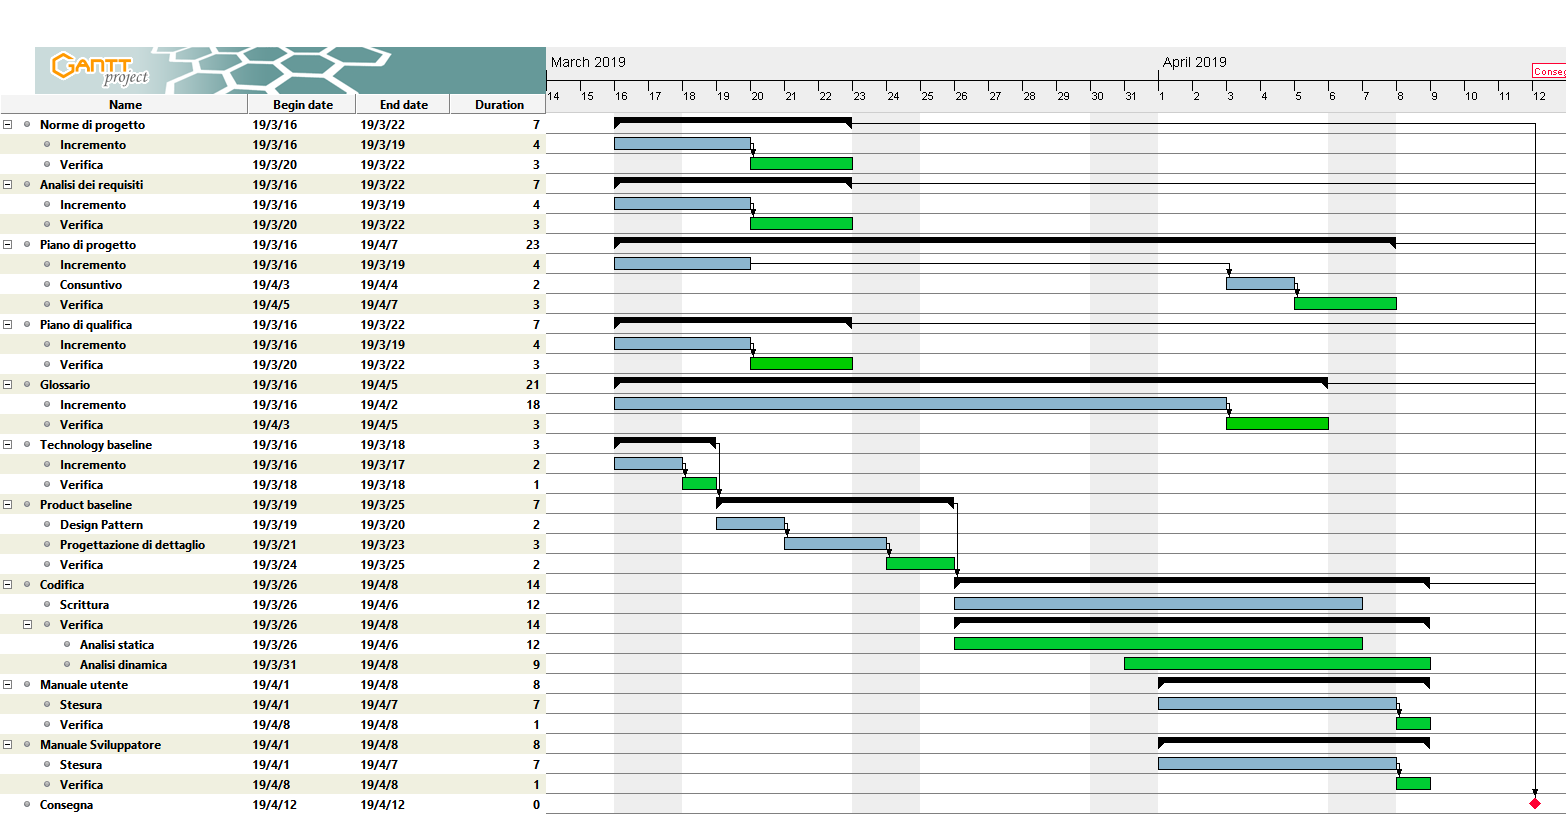
\includegraphics[scale=0.35]{Res/Gantt/Codifica}
	\caption{Diagramma dei casi d'uso}\label{}
\end{figure}

\pagebreak
